\chapter{Design}
\label{design}
The design phase is focused on game logic construction. It is based on previous chapters analysis and discoveries from articles connected with the topic of haptic rehabilitation for DCD, especially \cite{13}.

\section{Basic game rules and objects}
As it was previously described in \emph{\ref{rules} - \nameref{rules}}, the main task performed by patients is to follow the three-dimensional wire with tip of stylus, where the path is magnetically attractive. There is an object that player has to move from "start" to "end" along the path by pushing it with the tip of stylus, represented by cursor. There is also a competitor's object, moving along the path with uniform velocity (specified for each curve). The player wins a round when his object reaches the end before competitor's one. 

\subsection{Path}
The mathematical representation of this path is Bezier's curve. Depending on level of difficulty there are different curves - they vary in length, curvature and torsion. The are three designed curves. Each curve has defined two times of passing - one for slower and one for faster race. The competitor's speed is calculated based on this time and the current path length. 

\subsection{Haptic objects and displayed objects}
Terms "haptic" or "displayed" are used to describe object's visibility for haptic device. Only some of game's objects are rendered to haptic space and can be detected by the player while moving stylus through the space. Those are called haptic objects.

The haptic objects are:
\begin{itemize} [noitemsep, topsep={0pt}]
\item the path,
\item the player's object.
\end{itemize}
None of the other objects (i.e. competitor's object, "start" sign) is available to be detected by touch, they are only displayed on the screen. All of the haptic objects are also displayed one.

\begin{wrapfigure}[18]{L} {0.5\textwidth}
\begin{center}
	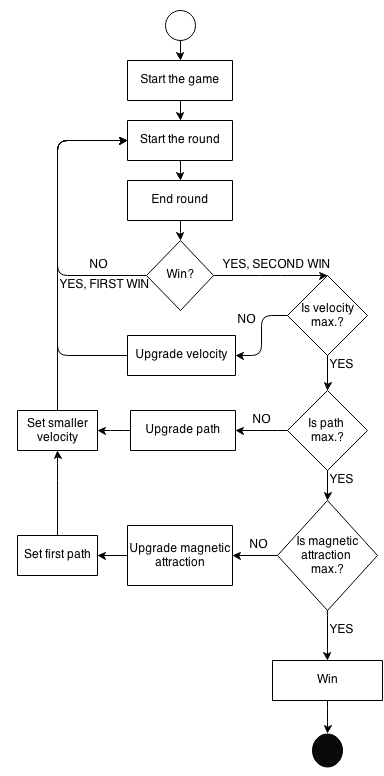
\includegraphics[height=12cm]{Images/leveling}
	\label{fig:leveling}	
	\caption{Schema of levelling process}
\end{center}
\end{wrapfigure}

\section{Levelling up}
There are three parameters that are changing along the game:
\begin{itemize} [noitemsep, topsep={0pt}]
\item the competitor's velocity,
\item the path's shape (and length),
\item the magnetic attraction level.
\end{itemize}
The player advances to the next level when he wins two times in a row with definite settings. While advancing, firstly, the competitor's velocity is increased. Then, when the player wins with both competitors, slow and fast one, he change the path to more advance, but with slower competitor again. Finally, after winning games on all paths, the magnetic attraction level is decreased and player starts from the very first path with slower competitor. This process is repeated until reaching the lowest possible level of magnetic attraction and is presented in \emph{\ref{fig:leveling} - \nameref{fig:leveling}}.

\section{Controls}
There are three possible input devices: a keyboard, a mouse and the Phantom Omni. The player's object is controlled only with a Phantom Omni to avoid the possible confusion. The mouse allows changing of camera position. The keyboard is reserved for debug operations (turning on and off scene's objects, immediate winning of round). 

\section{Display and scene}
The scene is closed in a skybox, a cube where inner walls are covered with textures. The path is rendered in the middle of the scene. Player's and competitor's object are attached to the path, so do start/end sign. There is also a graphic representation of a tip of a stylus. 

\section{Measuring player's score}
Continuous measuring player's score during a game is one of the most important parts of the project, as it allows to control his progress. There are two main values measured during the game: \emph{path length} (of the player's object) and \emph{total race time}.

The path length may differ from curve length in case player leaves the "magnetic field" of a wire. This affect more often children with dyspraxia. This parameter decreases while trainings and therefore is index of progress. The path length is sampled with approximately 50-60 Hz frequency.

Total race time is a parameter responsible for determining of win. The counting starts from the moment when player's object moves for a first time in a round and lasts until reaching the end point.	